\section{Digital Tools to aid the Elicitation Process}
\label{sec:digital_tools}
A suite of Python-based tools (using Qt5) was developed to support the elicitation process across three key stages. These interactive prototypes were deemed essential by all experts for visualizing and refining inputs. Future iterations will be released as open-source software to assist similar processes.
    
The first graphical tool was used to support the qualitative indicator elicitation. Following the logic detailed in \ref{sec:qualitative_indicators_uncertanty}, experts were first presented with the possibility of modifing the author's ranking (Figure \ref{fig:qi_order}). Then, a linear value function can be adjusted to increase or decrease the difference between alternatives (Figure \ref{fig:qi_value}).

The second tools was used for the value function elicitation of quantiative indicators (igure \ref{fig:value_function_elicitation}). This tool was developed to assist the mid-value splitting technique. This proved to be useful in the "first elicitation" but presented limitations in the subsequent elicitations where experts were asked to refine existing value functions. In this case, the experts felt that being tied to alter the 0.25, 0.5 and 0.75 indifference points was too restrictive. Future versions of the software might evaluate to allow more flexibility in this regard.

The final tool, developed for weight elicitation (Figure \ref{fig:weights_elicitation}), significantly simplified this inherently complex task by providing graphical for both the expert and the analyist. It also incorporated an "on-the-fly" consistency check that monitored ordinal consistency within each group. The interface highlighted compliant and non-compliant regions through slider coloring and boundary arrows, allowing analysts to immediately spot inconsistencies. This design offers flexibility: minor inconsistencies can be corrected in real time, while substantial discrepancies prompt the analyst to rephrase questions and request expert revisions without interrupting the elicitation workflow.

\begin{figure}[!ht]
    \centering
    \begin{minipage}{0.85\textwidth}
        \centering
        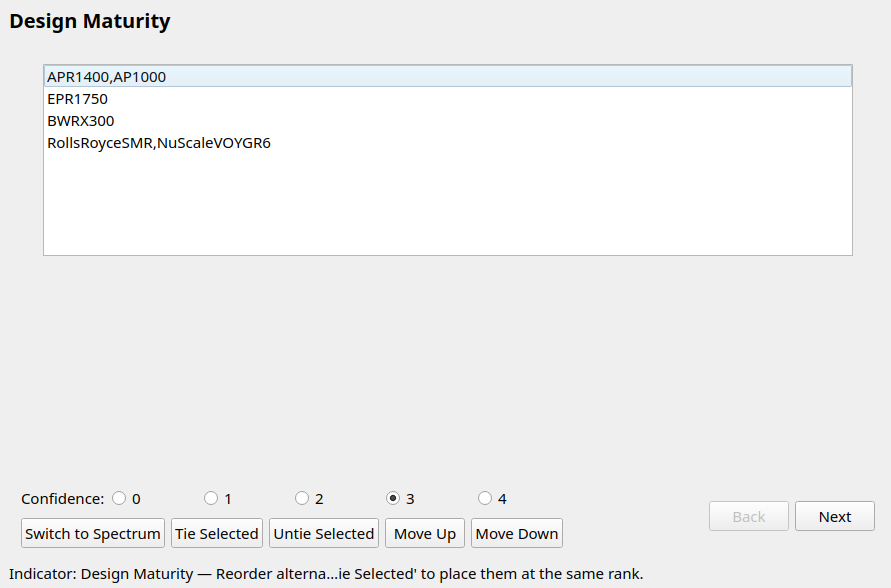
\includegraphics[width=\textwidth]{./imgs/QI_rank.png}
        \captionof{figure}{Ranking screen.}
        \label{fig:qi_order}
    \end{minipage}

    \vspace{0.75em}

    \begin{minipage}{0.85\textwidth}
        \centering
        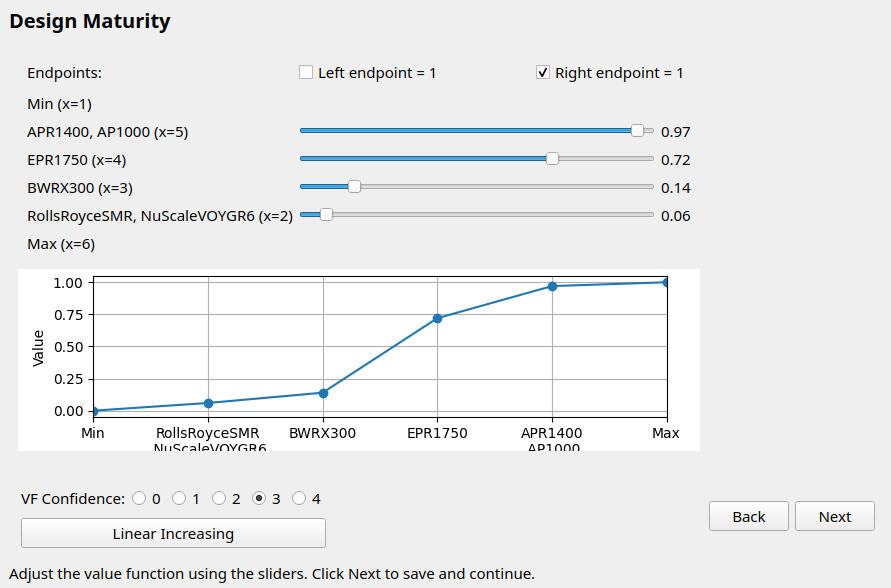
\includegraphics[width=\textwidth]{./imgs/QI_vf.png}
        \captionof{figure}{Value function screen.}
        \label{fig:qi_value}
    \end{minipage}
    \caption{Graphical interface for the elicitation of qualitative indicators.}
    \label{fig:qi_elicitation}
\end{figure}

\begin{figure}[htbp]
    \centering
    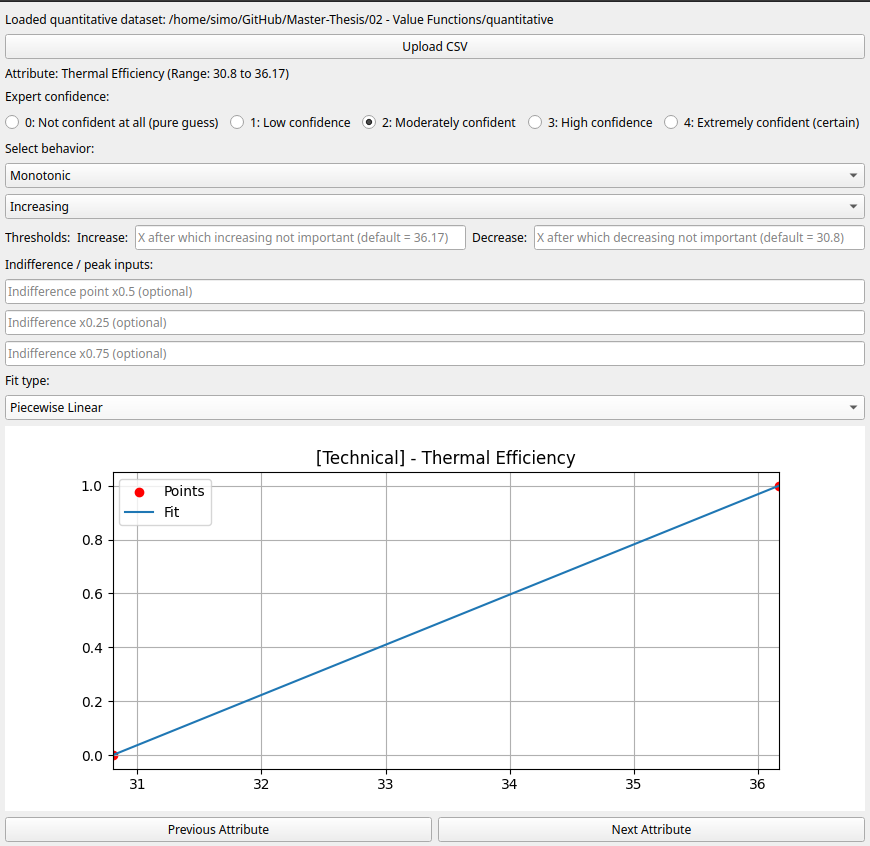
\includegraphics[width=0.75\textwidth]{./imgs/vf_UI.png}
    \caption{Value function elicitation interface showing mid-value splitting technique implementation.}
    \label{fig:value_function_elicitation}
\end{figure}

\begin{figure}[htbp]
    \centering
    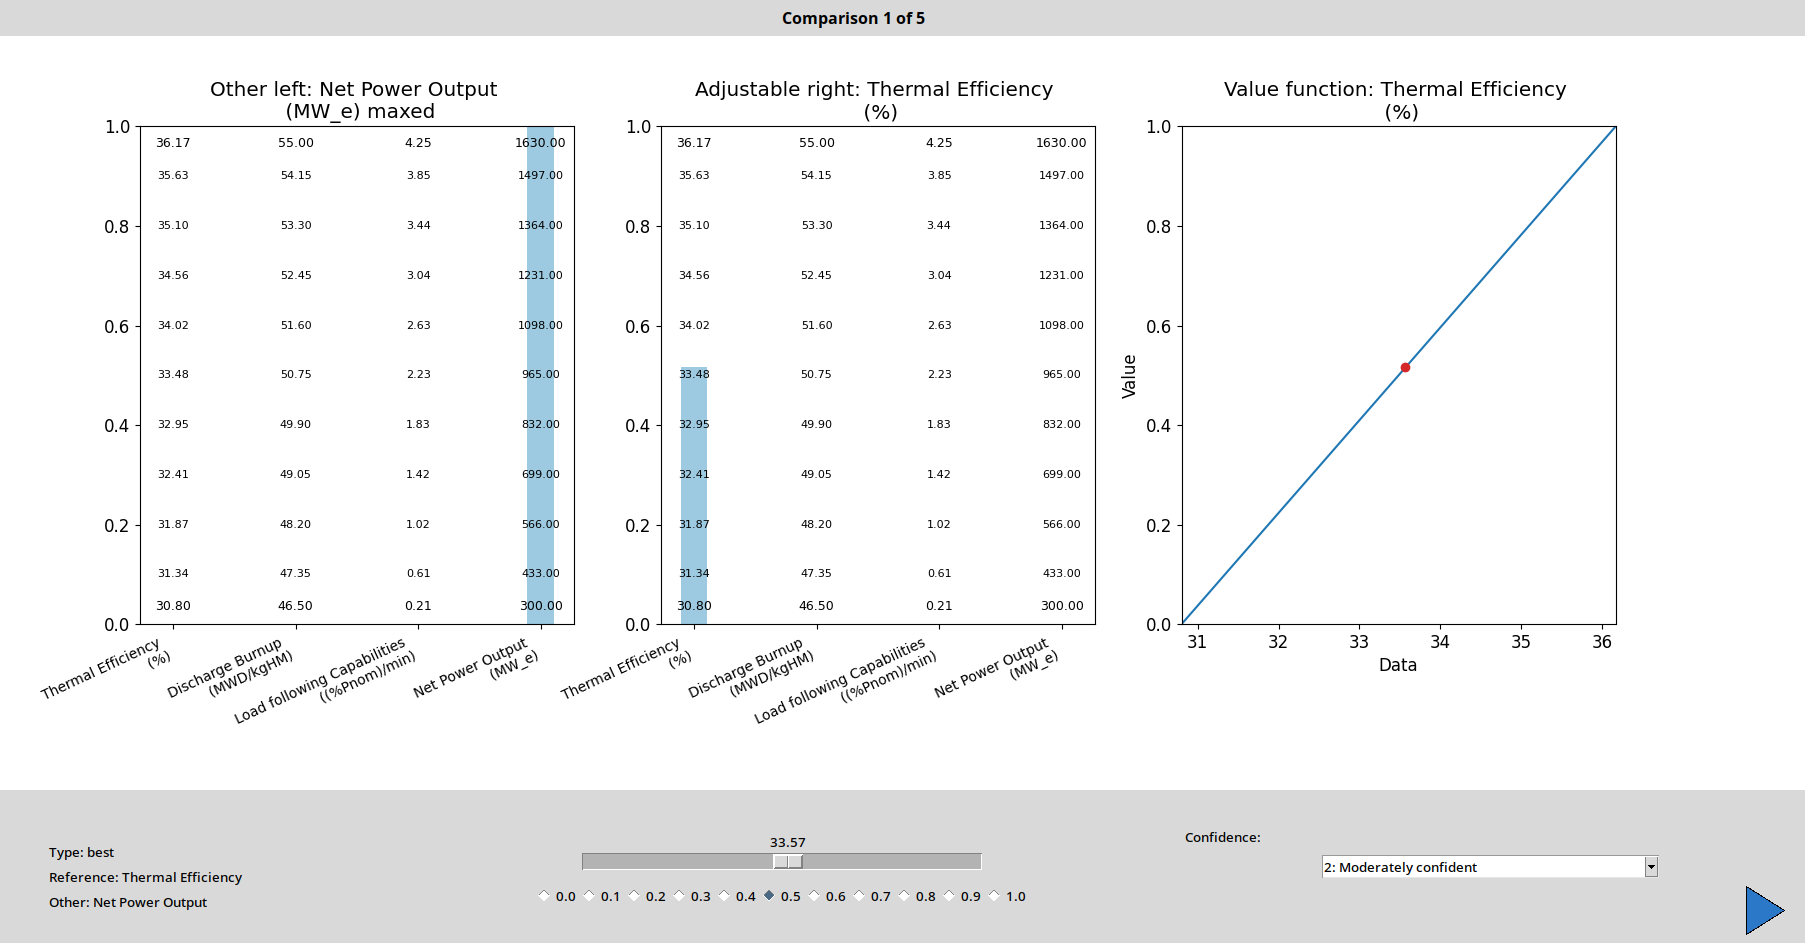
\includegraphics[width=0.8\textwidth]{./imgs/bwt_UI.png}
    \caption{Weights elicitation interface showing \gls{bwt} implementation.}
    \label{fig:weights_elicitation}
\end{figure}